\documentclass{article}
\usepackage{graphicx}
% \usepackage[paperheight=16cm,paperwidth=12cm,textwidth=10cm]{geometry}
\usepackage{lipsum}
\usepackage[T2A]{fontenc}
% \usepackage[koi8-r]{inputenc}
\usepackage[utf8]{inputenc}

\graphicspath{ {./Results/} }

\title{Merge Sort}
\author{Dadmo}
\date{\today}

\begin{document}
\maketitle

\tableofcontents 
\section{Merge Sort}
MergeSort --- клас, який має реалiзованi 4 варiанти алгоритму сортування злиттям. 
\begin{enumerate}
    \item Рекурсивний (Top-Down MergeSort)
    \item Ітеративний (Bottom-Up MergeSort)
    \item Ітеративний з оптимiзацiями cutoff(-to-insertion), stop-if-already-sorted, eliminate-the-copy-to-the-auxiliary-array.
    \item Сотування злиттям для зв’язного списку
\end{enumerate}
\indent В моїй реалiзації Ітеративного сортування злиттям використовується менше порівнянь для реверсивно відсортованих списків.
\newline
\indent В моїй реалiзації Ітеративного сортування злиттям з оптимiзацiями массиви розміру між $80 \cdot 10^A$  та $90 \cdot 10^A$, де A --- const, сортуються не до кінця (Останні $c$ елементів) через оптимізацію eliminate-the-copy-to-the-auxiliary-array.
\newline
\indent Також реалiзовано порiвняльний аналiз (з даними рiзного розмiру) всiх чотирьох варiантiв
алгоритму сортування злиттям вiдносно часу виконання, кiлькостi проведених
порiвнянь, операцiй "копiювань" та використаної пам’ятi. Окрім цього є показ на скільки відстотків обрахунки вже завершено.
\newline
% \newline
\section{Random Lists}
RandomLists --- клас, який має реалiзованi 5 варiанти генерацiї спискiв.
\begin{enumerate}
    \item Повнiстю вiдсортований (sorted) --- на вхід подається лише розмiр списку.
    \item Випадковi (random) --- на вхід подається лише розмiр списку.
    \item Майже вiдсортований (almostsorted) --- на вхід подається розмiр списку, та відсоток безпорядку.
    \item Вiдсортованi в зворотному порядку (reverse) --- на вхід подається лише розмiр списку.
    \item Лише з декiлькома рiзними значеннями (somenumbers) --- на вхід подається розмiр списку, та діапазон значень (Початок, Кiнець).
\end{enumerate}
\section{Linked Lists}  

    \indent Node --- клас, який зберігає дані, а також посилання на наступний та попередній елементи.
    Для нього реалiзовано отримання розмiру в байтах, а також реалiзованi усі порівняння.

    LinkedList --- клас, який зберігає посилання на перший та останній елементи.
    Для нього реалiзовано отримання розмiру в байтах, а також реалiзоване
    додавання елементів, розширення списку, підрахунок певної підкількості елементів, а також видалення елементів.
    \newline
    \indent Додатково реалiзовано призначення та отримання елемента за індексом, слайсом індексів списку.
\section{Converters}
Converter --- клас, в якому реалiзовано конвертацiю масиву у зв’язний список та навпаки.
\section{Comparisions and Results}
    Подивимося результати виконання. Розміри масивів: від 10 до 10000 елементів з кроком в 100.
    \newline
    \subsection{Спочатку для відсортованих масивів:}
    Час виконання:
    \newline
        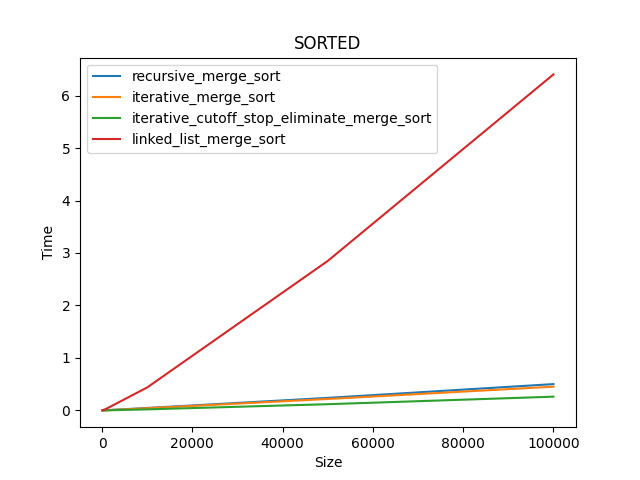
\includegraphics[scale=0.5]{sorted_Time_4_sorts_6_numbers_50_100to100000.png}
        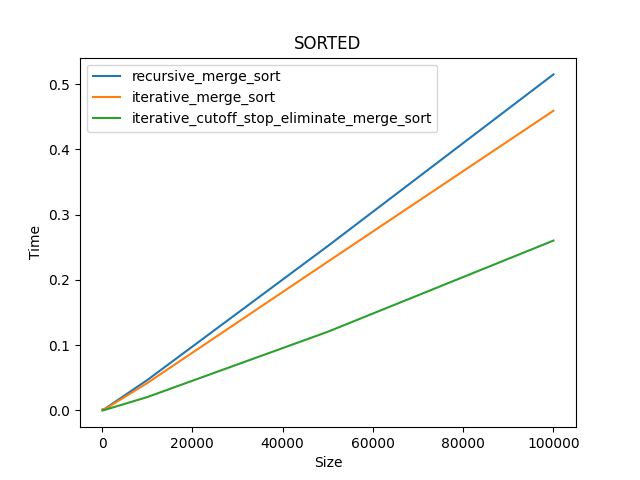
\includegraphics[scale=0.5]{sorted_Time_3_sorts_6_numbers_50_100to100000.png}
    \newline
    Кiлькiсть проведених порiвнянь:
    \newline
        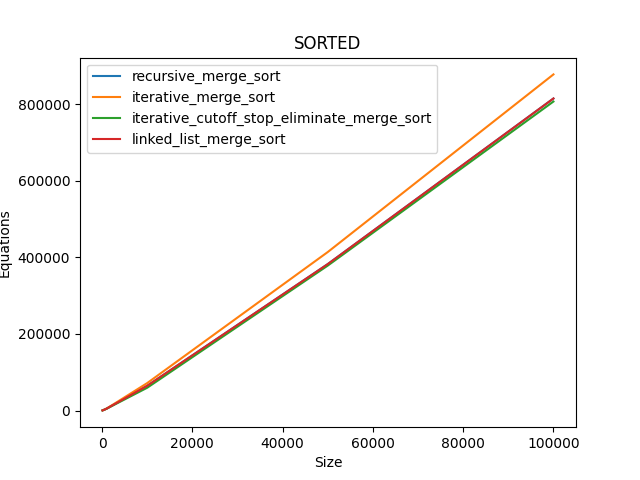
\includegraphics[scale=0.5]{sorted_Equations_4_sorts_6_numbers_50_100to100000.png}
        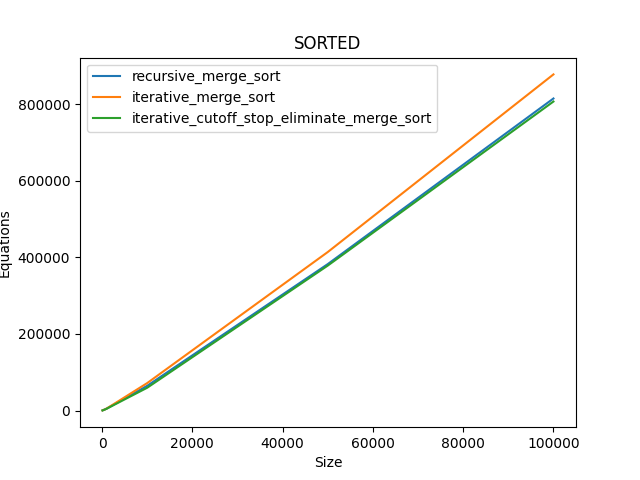
\includegraphics[scale=0.5]{sorted_Equations_3_sorts_6_numbers_50_100to100000.png}
    \newpage
    Операцiї "копiювань":
    \newline
        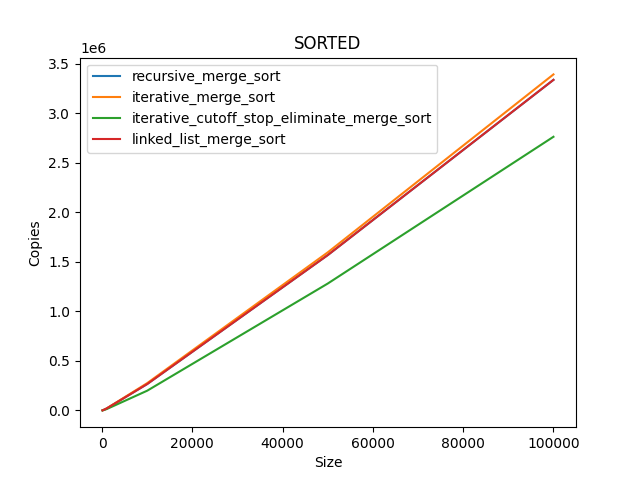
\includegraphics[scale=0.5]{sorted_Copies_4_sorts_6_numbers_50_100to100000.png}
        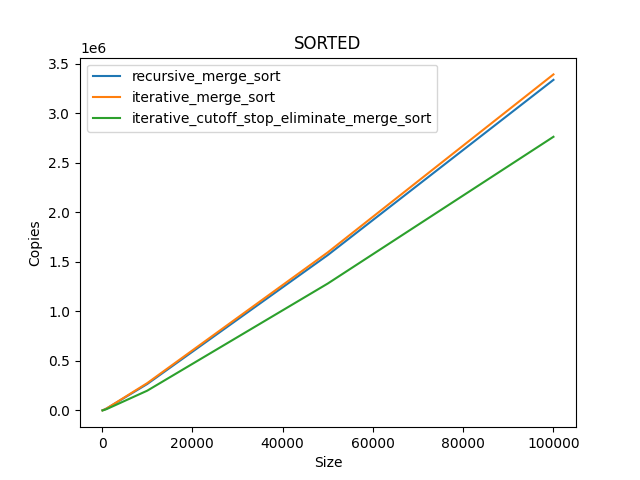
\includegraphics[scale=0.5]{sorted_Copies_3_sorts_6_numbers_50_100to100000.png}
    \newline
    Використано пам’ятi:
    \newline
        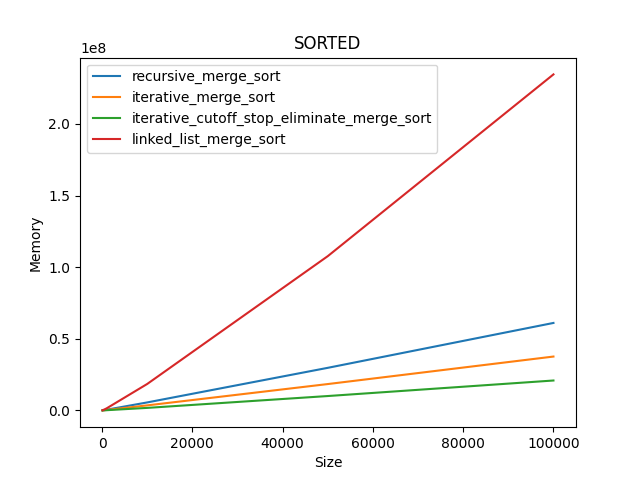
\includegraphics[scale=0.5]{sorted_Memory_4_sorts_6_numbers_50_100to100000.png}
        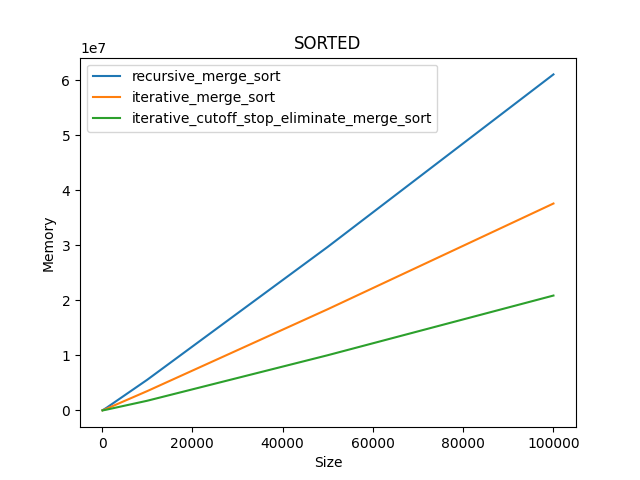
\includegraphics[scale=0.5]{sorted_Memory_3_sorts_6_numbers_50_100to100000.png}
    \newpage
    \subsection{Потім для масивів випадкових значень:} 
    Час виконання:
    \newline
        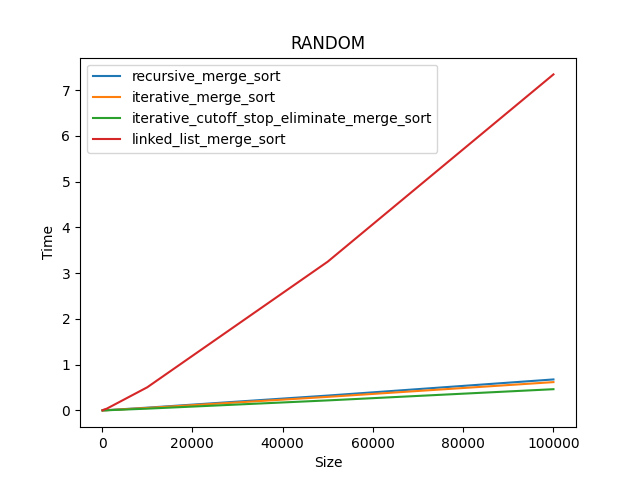
\includegraphics[scale=0.5]{random_Time_4_sorts_6_numbers_50_100to100000.png}
        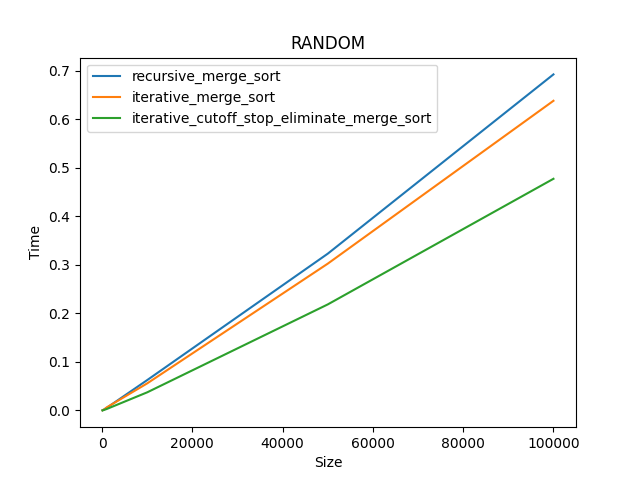
\includegraphics[scale=0.5]{random_Time_3_sorts_6_numbers_50_100to100000.png}
    \newline
    Кiлькiсть проведених порiвнянь:
    \newline
        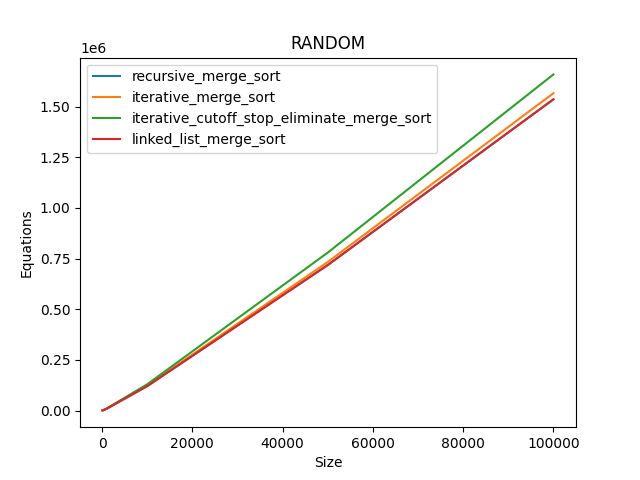
\includegraphics[scale=0.5]{random_Equations_4_sorts_6_numbers_50_100to100000.png}
        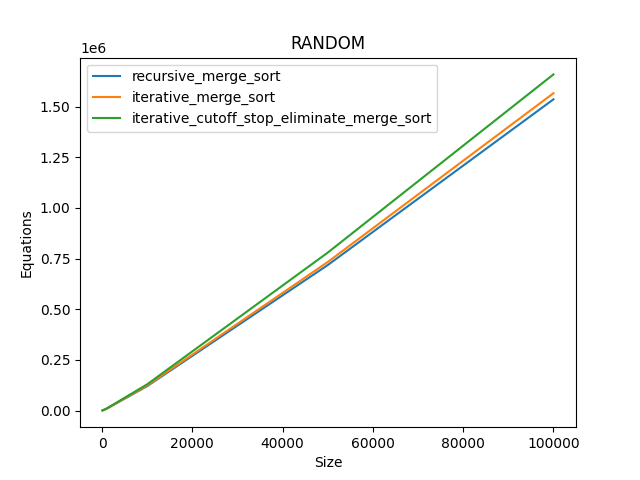
\includegraphics[scale=0.5]{random_Equations_3_sorts_6_numbers_50_100to100000.png}
    \newpage
    Операцiї "копiювань":
    \newline
        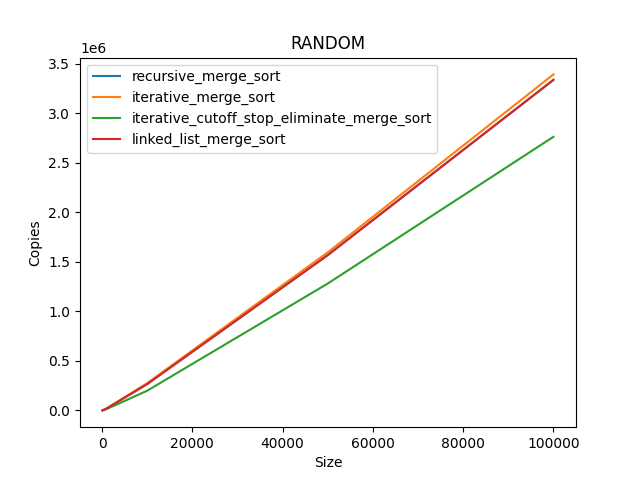
\includegraphics[scale=0.5]{random_Copies_4_sorts_6_numbers_50_100to100000.png}
        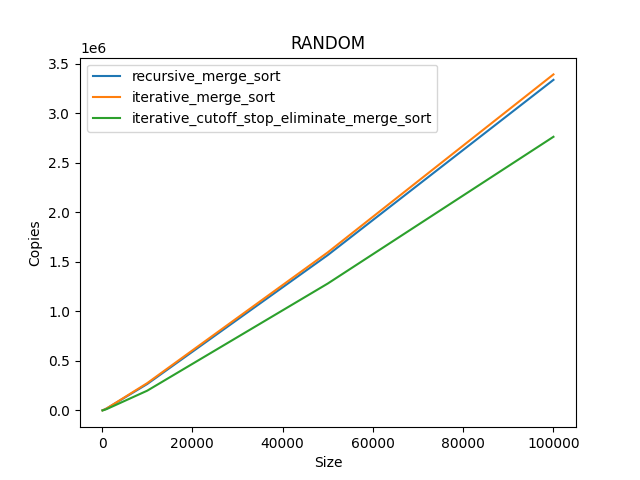
\includegraphics[scale=0.5]{random_Copies_3_sorts_6_numbers_50_100to100000.png}
    \newline
    Використано пам’ятi:
    \newline
        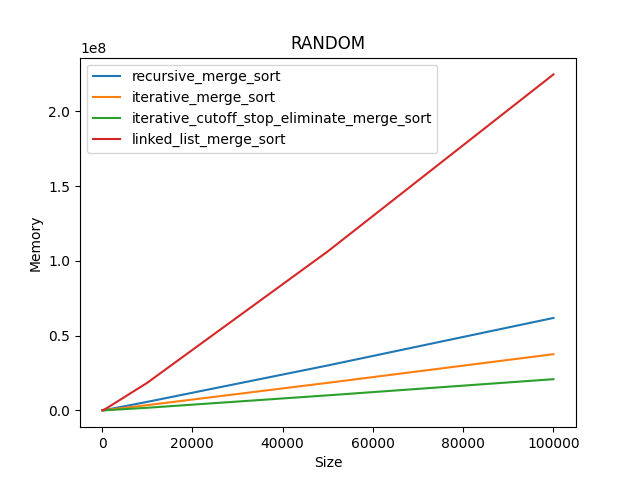
\includegraphics[scale=0.5]{random_Memory_4_sorts_6_numbers_50_100to100000.png}
        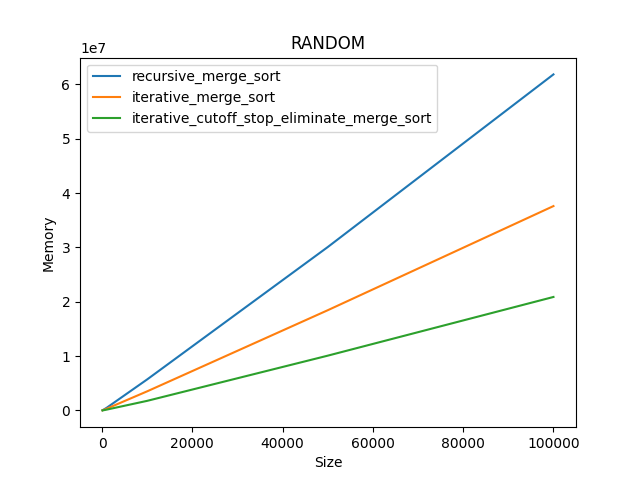
\includegraphics[scale=0.5]{random_Memory_3_sorts_6_numbers_50_100to100000.png}
    \newpage
    \subsection{Масив майже відсортованих значень:}
    Час виконання:
    \newline
        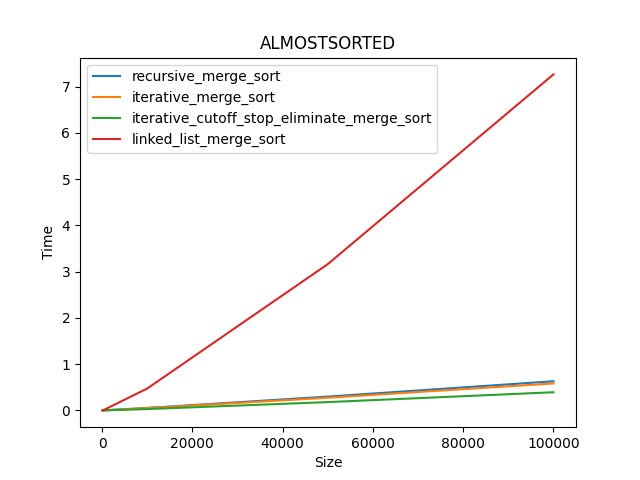
\includegraphics[scale=0.5]{almostsorted_Time_4_sorts_6_numbers_50_100to100000.png}
        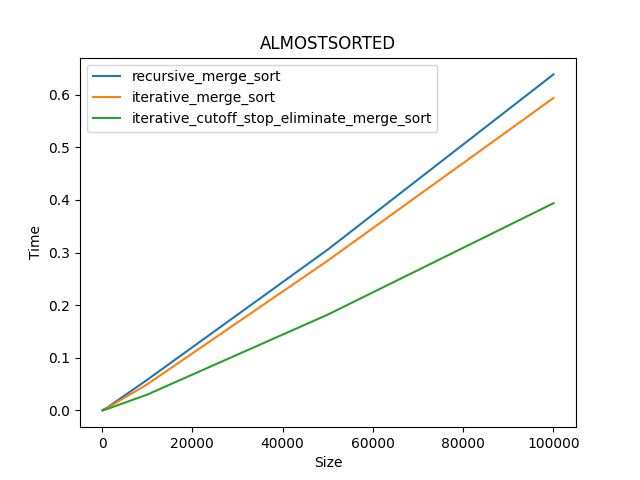
\includegraphics[scale=0.5]{almostsorted_Time_3_sorts_6_numbers_50_100to100000.png}
    \newline
    Кiлькiсть проведених порiвнянь:
    \newline
        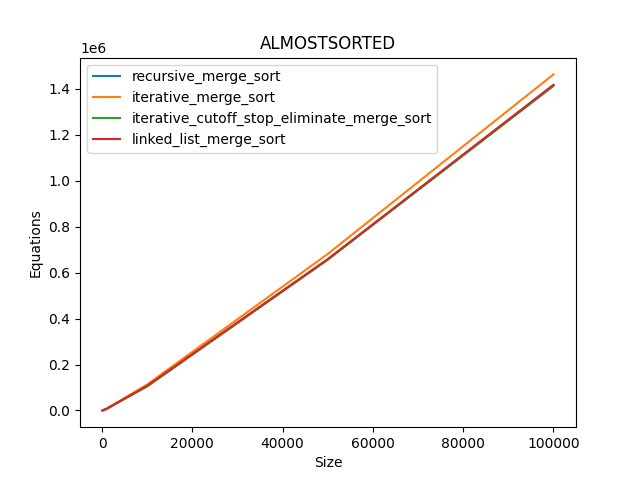
\includegraphics[scale=0.5]{almostsorted_Equations_4_sorts_6_numbers_50_100to100000.png}
        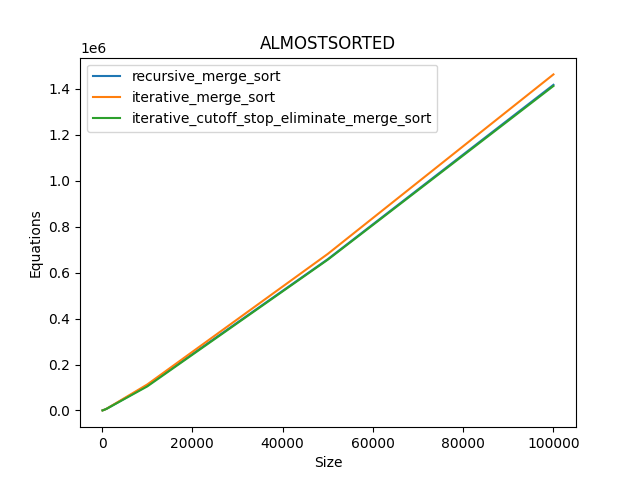
\includegraphics[scale=0.5]{almostsorted_Equations_3_sorts_6_numbers_50_100to100000.png}
    \newpage
    Операцiї "копiювань":
    \newline
        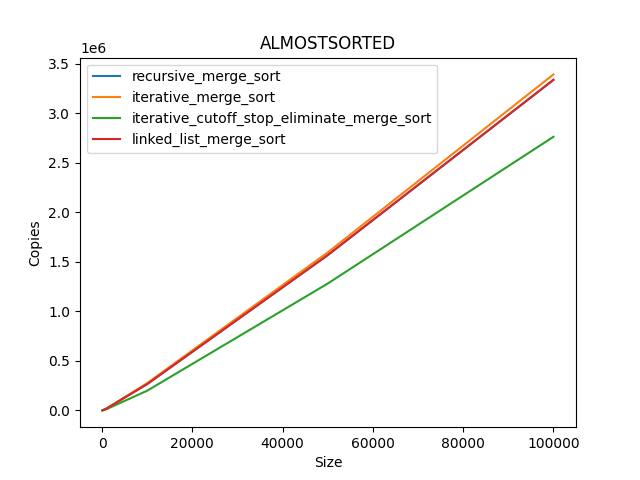
\includegraphics[scale=0.5]{almostsorted_Copies_4_sorts_6_numbers_50_100to100000.png}
        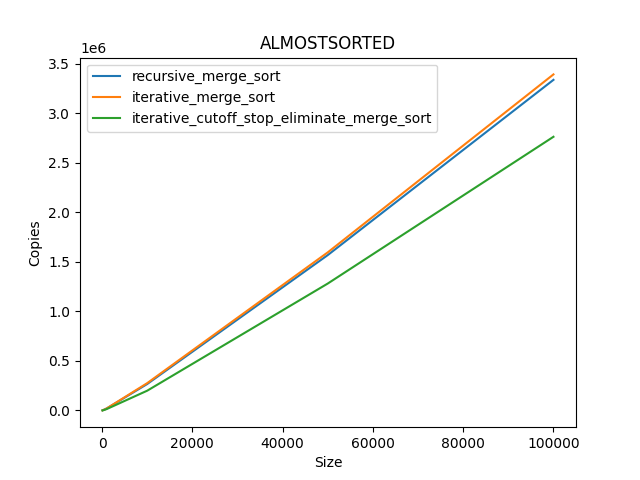
\includegraphics[scale=0.5]{almostsorted_Copies_3_sorts_6_numbers_50_100to100000.png}
    \newline
    Використано пам’ятi:
    \newline
        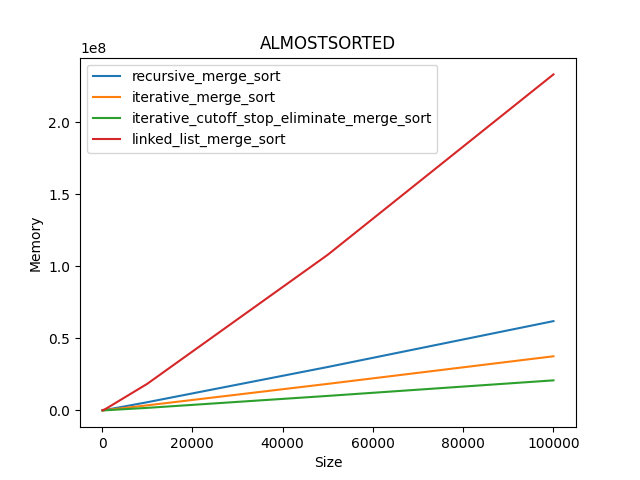
\includegraphics[scale=0.5]{almostsorted_Memory_4_sorts_6_numbers_50_100to100000.png}
        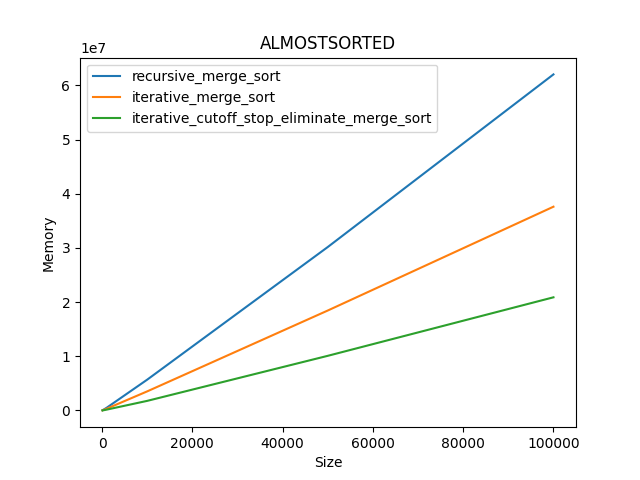
\includegraphics[scale=0.5]{almostsorted_Memory_3_sorts_6_numbers_50_100to100000.png}
    \newpage
    \subsection{Масив відсортованих значень у зворотному порядку:}
    Час виконання:
    \newline
        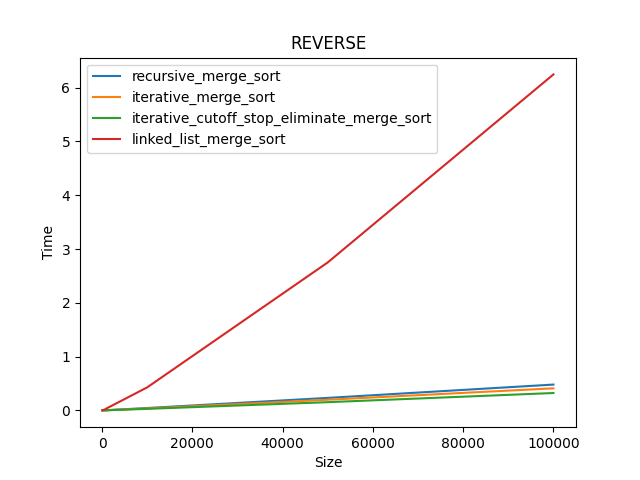
\includegraphics[scale=0.5]{reverse_Time_4_sorts_6_numbers_50_100to100000.png}
        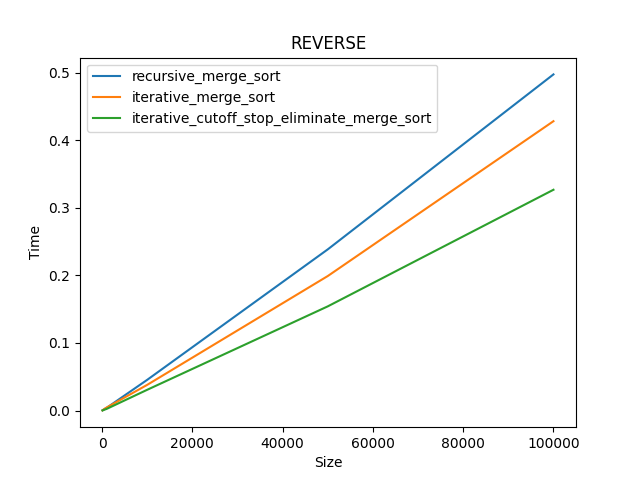
\includegraphics[scale=0.5]{reverse_Time_3_sorts_6_numbers_50_100to100000.png}
    \newline
    Кiлькiсть проведених порiвнянь:
    \newline
        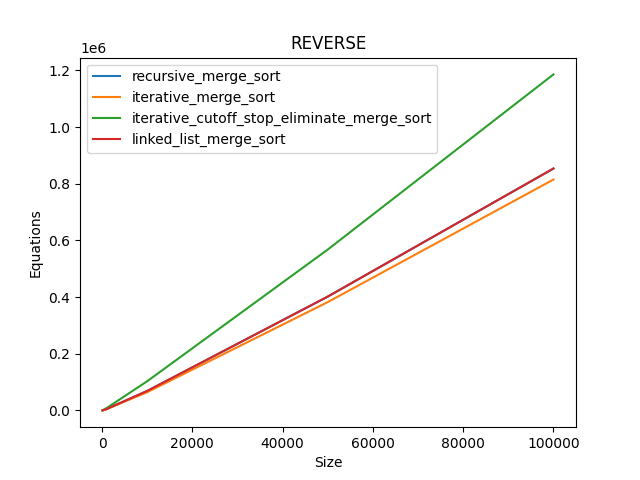
\includegraphics[scale=0.5]{reverse_Equations_4_sorts_6_numbers_50_100to100000.png}
        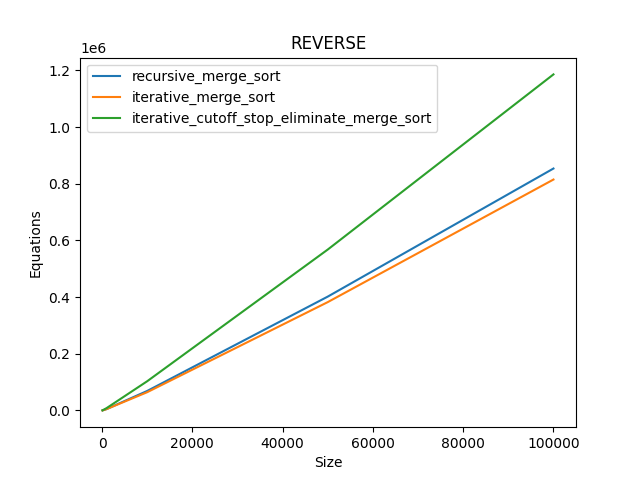
\includegraphics[scale=0.5]{reverse_Equations_3_sorts_6_numbers_50_100to100000.png}
    \newpage
    Операцiї "копiювань":
    \newline
        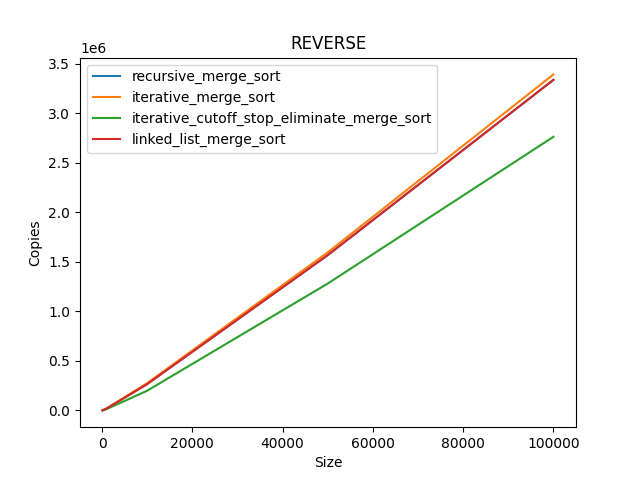
\includegraphics[scale=0.5]{reverse_Copies_4_sorts_6_numbers_50_100to100000.png}
        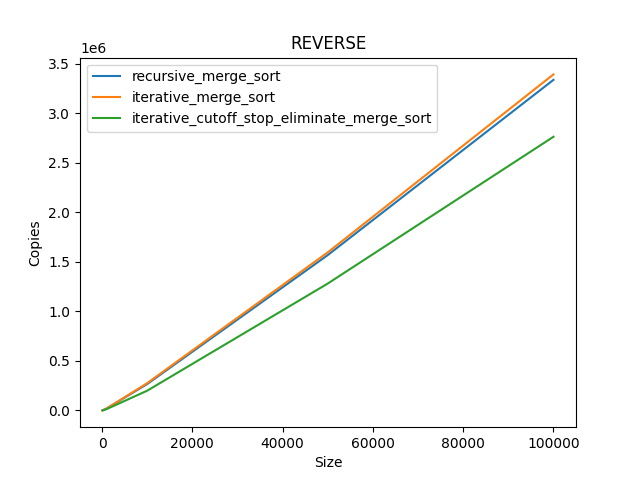
\includegraphics[scale=0.5]{reverse_Copies_3_sorts_6_numbers_50_100to100000.png}
    \newline
    Використано пам’ятi:
    \newline
        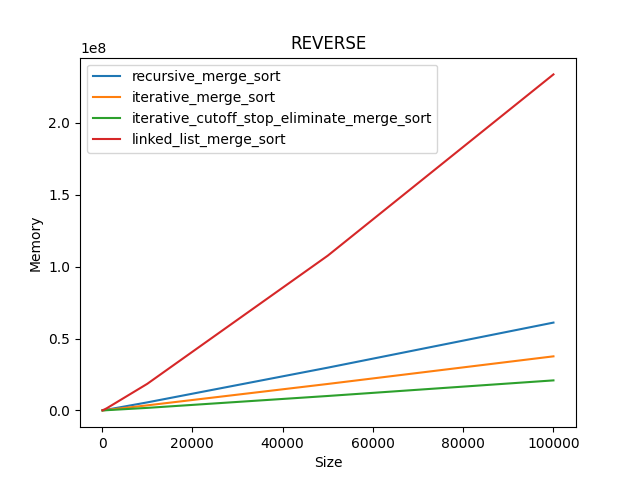
\includegraphics[scale=0.5]{reverse_Memory_4_sorts_6_numbers_50_100to100000.png}
        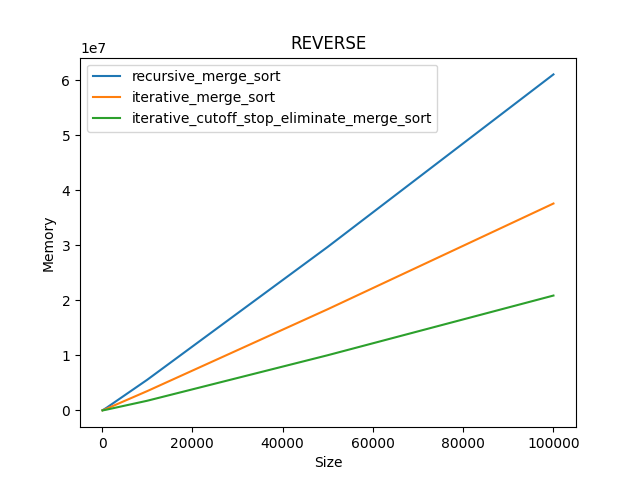
\includegraphics[scale=0.5]{reverse_Memory_3_sorts_6_numbers_50_100to100000.png}
    \newpage
    \subsection{Масив тільки з декiлькома рiзними значень:}
    Час виконання:
    \newline
        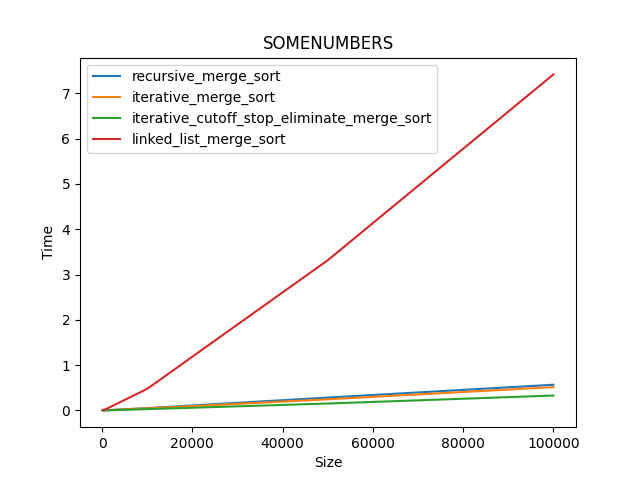
\includegraphics[scale=0.5]{somenumbers_Time_4_sorts_6_numbers_50_100to100000.png}
        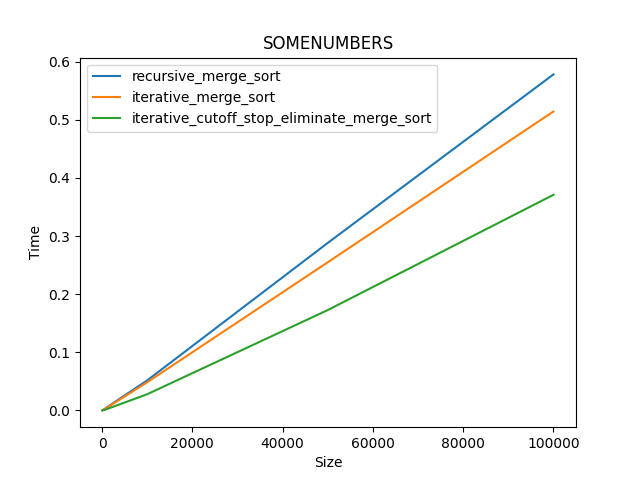
\includegraphics[scale=0.5]{somenumbers_Time_3_sorts_6_numbers_50_100to100000.png}
    \newline
    Кiлькiсть проведених порiвнянь:
    \newline
        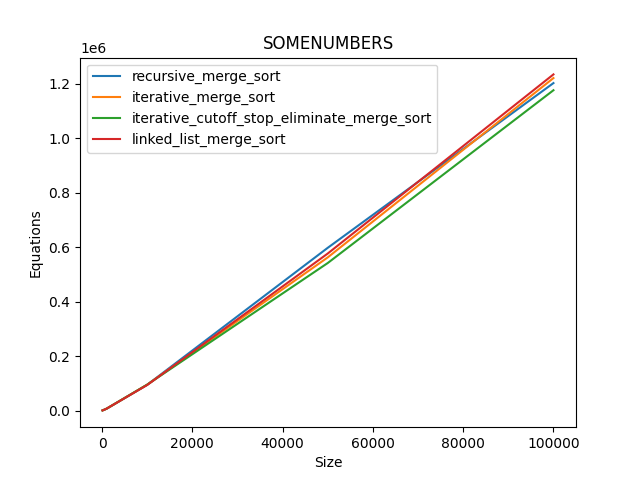
\includegraphics[scale=0.5]{somenumbers_Equations_4_sorts_6_numbers_50_100to100000.png}
        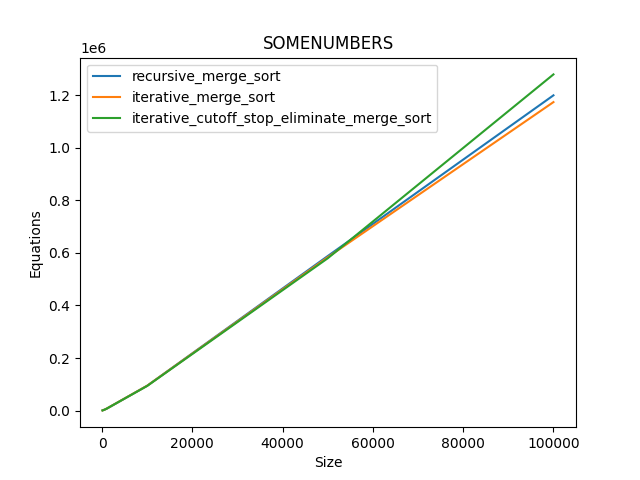
\includegraphics[scale=0.5]{somenumbers_Equations_3_sorts_6_numbers_50_100to100000.png}
    \newpage
    Операцiї "копiювань":
    \newline
        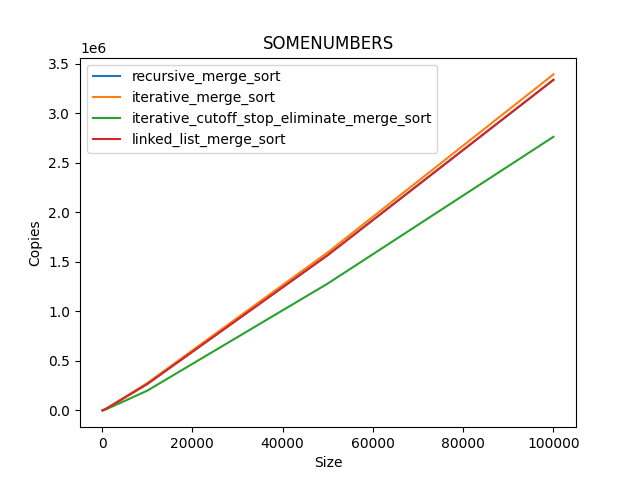
\includegraphics[scale=0.5]{somenumbers_Copies_4_sorts_6_numbers_50_100to100000.png}
        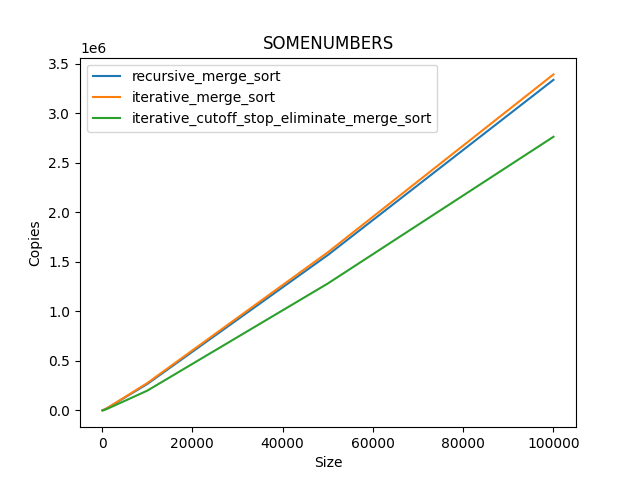
\includegraphics[scale=0.5]{somenumbers_Copies_3_sorts_6_numbers_50_100to100000.png}
    \newline
    Використано пам’ятi:
    \newline
        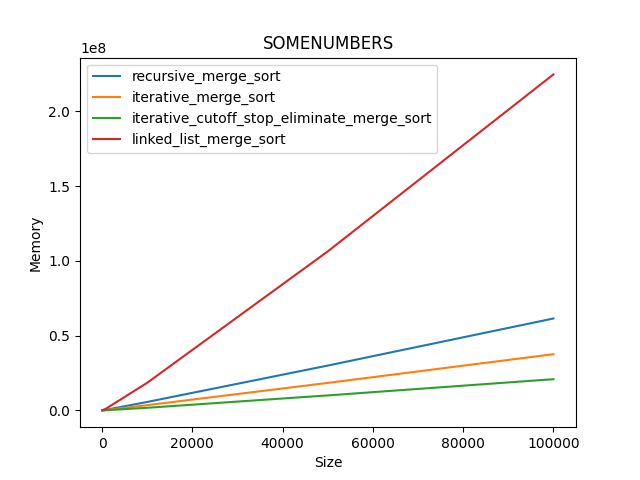
\includegraphics[scale=0.5]{somenumbers_Memory_4_sorts_6_numbers_50_100to100000.png}
        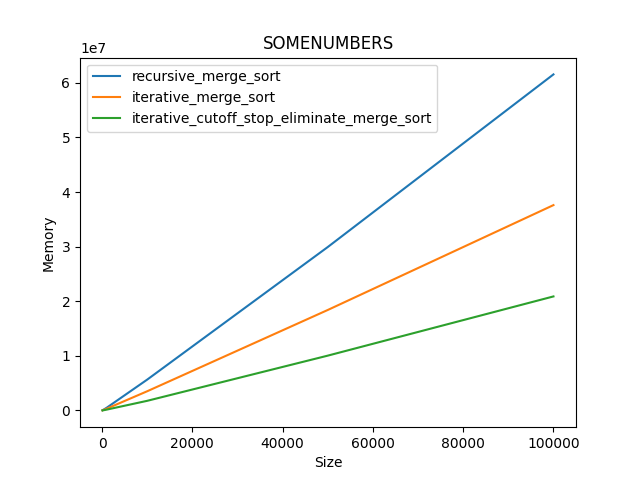
\includegraphics[scale=0.5]{somenumbers_Memory_3_sorts_6_numbers_50_100to100000.png}
    \newpage
    \subsection{Results:}
    \begin{enumerate}
        \item Час виконання --- сортування злиттям для спискiв завжди має найбільший час виконання через те, як я їх реалізував.
        \item Час виконання --- Найшвидшим завжди є ітеративний з оптимізаціями.
        \item Кiлькiсть проведених порiвнянь --- Ітеративний без оптимізацій завжди має найбільшу кiлькiсть порiвнянь для відсортованих масивів та завжди має найменшу кiлькiсть порiвнянь для відсортованих у зворотному порядку масивів.
        \item Кiлькiсть проведених порiвнянь --- Ітеративний з оптимізаціями завжди має найбільшу кiлькiсть порiвнянь для відсортованих у зворотному порядку масивів.
        \item Операцiї "копiювань" --- у ітеративного з оптимiзацiями завжди менше всіх.
        \item Пам'ять ---  завжди однакова.
    \end{enumerate}
\end{document}

% 4. Оформлення результатiв роботи та звiту
% Результатом роботи є всi тексти програм, за потреби скомпiльованi виконуванi файлi (якi
% мають запускатися на чистiй ОС; якщо є потреба, можна використовувати контейнери), необхiдна
% документацiя щодо використання з прикладами застосування та звiт.
% Звiт до комп’ютерного практикуму оформлюється згiдно зi стандартними правилами
% оформлення наукових робiт. Тексти програм не включати у звiт.